\section{Evaluation for Pockels effects}
In this section, we calculate the electro-optic coefficient 
by two methods, using the result of the theoretical part, given by
\begin{equation}
    r_{41} = \frac{\lambda d}{4 l U_{\lambda / 2}} 
    \left(\frac{1}{2} \left(\frac{1}{\eps_\perp} + \frac{1}{\eps_\parallel}\right)\right)^{\frac{3}{2}}\, .
    \label{eq:r_41_U}
\end{equation}

If we take the values given in section \ref{tab:pockels_technical}, 
and estimate the uncertainties, we get the following parameters:
\begin{itemize}
\setlength\itemsep{0em}
\item[] $\lambda = (632.8\pm 0.1)$nm
\item[] $n_1     = 1.522\pm 0.001$
\item[] $n_3     = 1.477\pm 0.001$
\item[] $l       = ( 20\pm 0.1)$mm
\item[] $d       = (2.4\pm 0.1)$mm
\end{itemize}

Now we can calculate $r_{41}$ with respect to $U_{\lambda/2}$ with two different methods.

\subsection{Saw tooth method}
\label{ssub:Saw tooth method}

\subsection{DC current method}
\label{ssub:DC current method}
As seen in the measurements section, the frequency doubling can be 
observed best for a frequency of the input sine signal with 
$0.5 kHz$. For the corresponding data sets, we use Fourier analysis 
described in~\ref{sec:pdf} to determine 
the input voltage $U_\mathrm{DC}$ at which frequency doubling occurs. 
To illustrate the procedure, we show an example at $U_\mathrm{DC} = 137.0$ V.
The cut-off is taken at $t = 1.1$ ms and $t = 9.05$ ms, as shown in figure 
\ref{fig:cut_off_example}. The result of the FFT is then shown in figure 
\ref{fig:fft_example} for a larger range of frequencies and those of interest, 
namly $\nu < 2$ kHz. One clearly observes the two peaks close to 
0.5 kHz and 1.0 kHz, being of the same scale. This procedure is 
done with all datasets corresponding to the signals shown in 
the figures \ref{fig:sinus8}, which has shown the largest 
change regarding frequency doubling by eye. The result of the fourier 
analysis in the range from $0$ to $2$ kHz as well as the 
value of $|\mathrm{FFT}\left[U_\mathrm{out} \left(\nu\right)\right]|^2$ for 
$\nu_1 = 0.45$ kHz and $\nu_2 = 0.91$ kHz 
is shown in figure \ref{fft_all}.
One can clearly observe the drop in amplitude for $U_\mathrm{DC} = 139.0$ kHz. 
We will thus take this to be our measured value for $\Ula$.
\begin{figure}
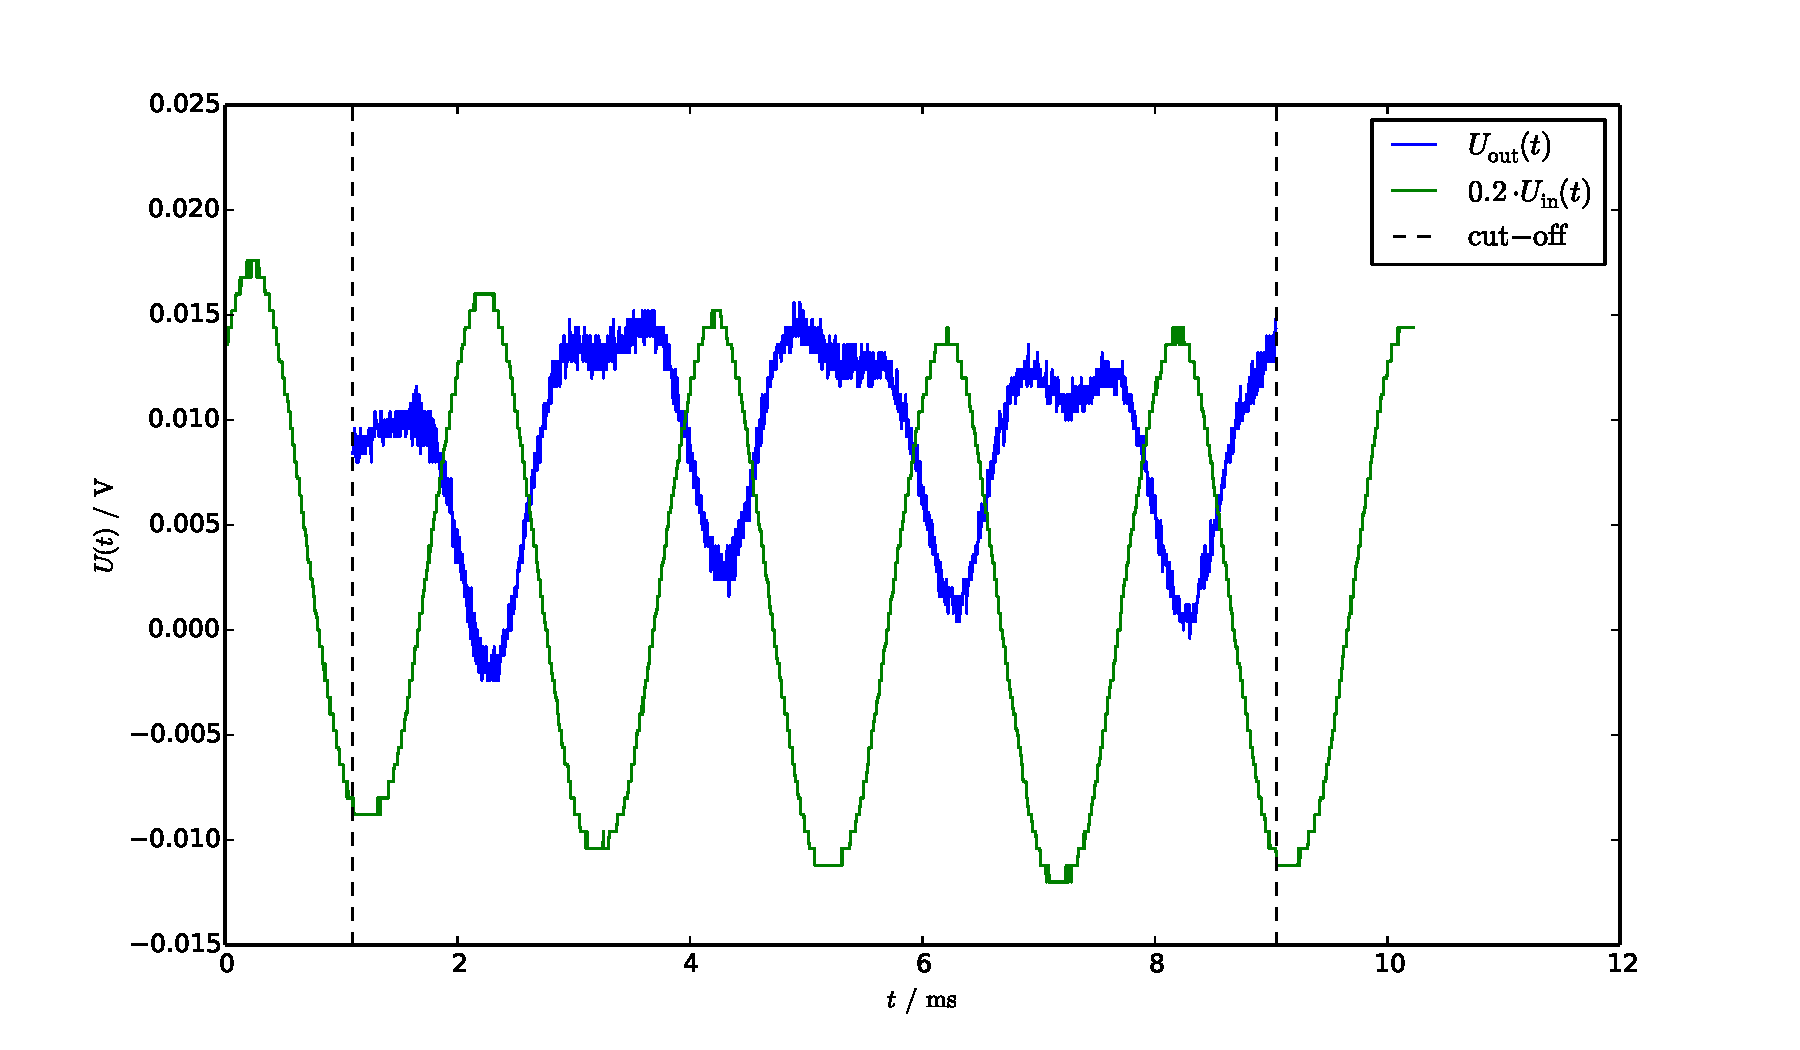
\includegraphics[width=\textwidth]{figures/cut_off_example.pdf}
\caption{
    Example for cut off points, for measured data at 
    $U_\mathrm{DC} = 137.0$ V. The minima of the input 
    signal $U_\mathrm{in}$, which is shown rescaled in this plos, 
    are found numerically in the ranges 
    $t \in (1.0, 1.5)$ ms and $t \in (8.5, 9.5)$ ms. 
    Further window functions are not applied. 
    By eye, the frequency doubling is seen already. 
    }
\label{fig:cut_off_example}
\end{figure}

\begin{figure}
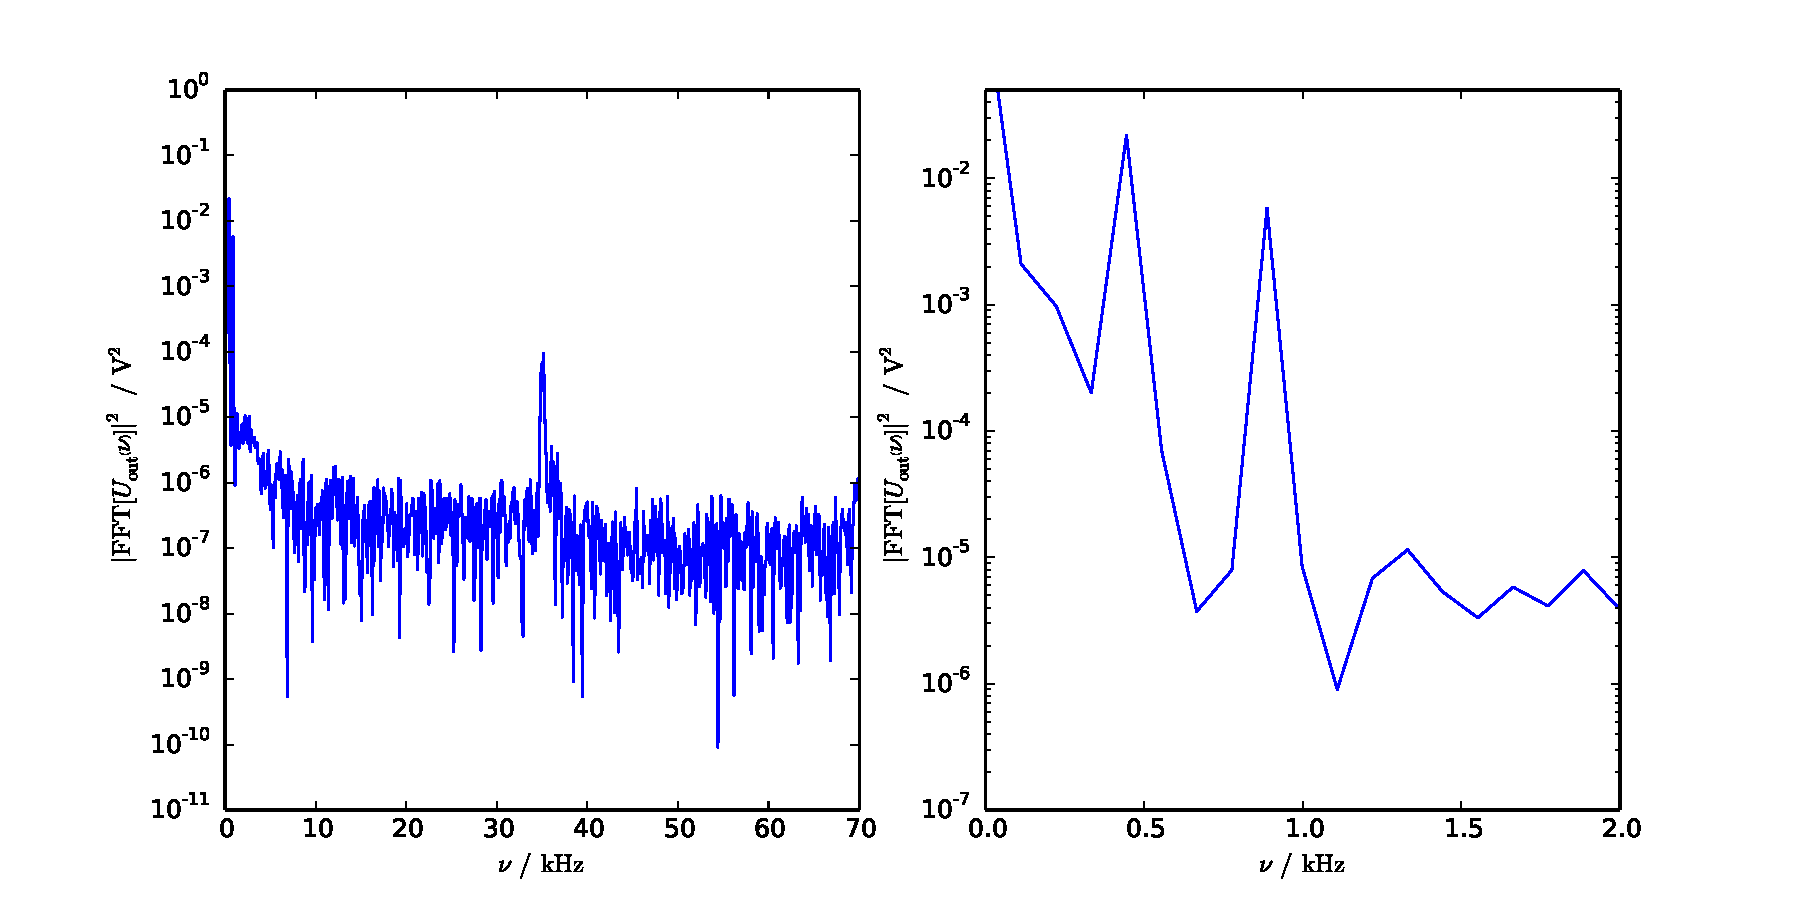
\includegraphics[width=\textwidth]{figures/fft_example.pdf}
\caption{
    Example for results of fourier analysis, for measured data at 
    $U_\mathrm{DC} = 137.0$ V.
    On the larger range, one observes strong peaks for low frequencies 
    and one relatively high peak at $\nu = 35.0$ kHz, which will not be 
    subject to further analysis. On the reduced range, the two peaks 
    due to the input signal and frequency doubling can be observed. 
    }
\label{fig:fourier_example}
\end{figure}

\begin{figure}
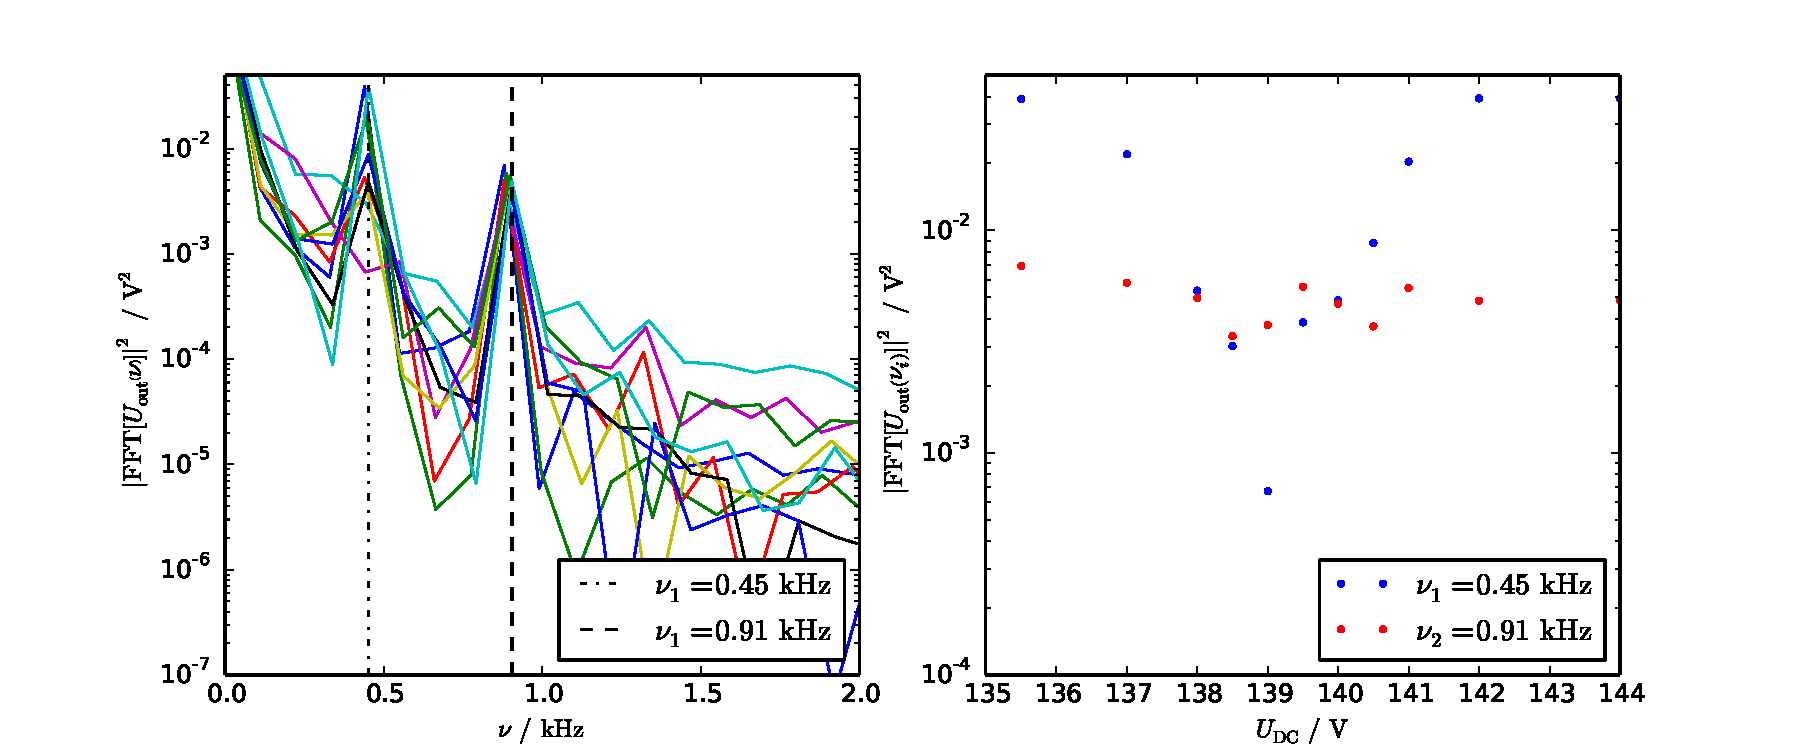
\includegraphics[width=1.0\textwidth]{figures/fft_all.pdf}
\caption{
    Taken the quantity
    $|\mathrm{FFT}\left[U_\mathrm{out} \left(\nu\right)\right]|^2$ 
    for all datasets yields a fairly confusing image, 
    which is, however, instructive as one observes the 
    frequency doubling for the different direct currents 
    $U_\mathrm{DC}$.
    In the right plot, the minimum for the lower frequency indicates 
    the maximal frequency doubling. We expected a maximum in the 
    double frequency, which clearly doesn't show. This 
    may be due to the small size of the dataset (in terms 
        of $t$ or the number of oscillations). 
    }
\label{fig:fft_all}
\end{figure}

The value of $\Ula$ for the given input signal is thus 
found with $\Ula = (135  \pm 15)$. 
The estimated the uncertainty on $\Ula$ based on the 
observation, that $\Ula$ appeared to be 
depending on the frequency. This phenomenon is not 
explained in the formalism used in the theoretical sections. 
Further, we expect quite large uncertainties due to 
electronic noise and offsets. 

Using the parameters given above, we get the following result: 
\begin{equation*}
r_{41} = \left (41.7 \pm 2.3 \right )  \mathrm{pm}
\end{equation*}
